%% ------------------------------------------------------------------------- %%
\chapter{Applications}
\label{cap:Applications}

%% ------------------------------------------------------------------------- %%
%\begin{itemize}
%\item Give a glance at what type of application we have, focus on 2 algorithimic
%\item Rabin Karp
%\item Hashing trees
%\end{itemize}
%% ------------------------------------------------------------------------- %%

Hash functions and hash tables have a great number of applications in computer science. During this last section I focus on applications of hash functions in algorithms, but citing superficially applications in other areas (like criptography, data deduplication and caching).

Among the applications that I explain in this section there is a focus in two applications: Rabin-Karp string matching algorithm and hashing of a rooted tree for isomorphism checking. Rabin-karp string matching algorithm is one of the main application of a technique called rolling hashing. Hahsing of rooted tree for isomorphism checking is an interesting application sometimes used in competitive programming.

To motivate the start of this thesis I will start using hash tables to solve a very simple, yet famous, problem called 3-sum.
\section{3-sum problem}
The problem is stated as following:

\medskip

\textquote{\textit{Make a function that given an array of integer numbers and an integer S, it returns if there are any 3 different elements in this array that its sum equals S. Assume that there are no three different elements in the array that overflow a 32-bit integer when summed together.}}

\medskip

This a very interesting problem that has many different solutions. To start I will show and explain to you the brute force solution:

\begin{lstlisting}
bool threeSumWithoutHashTable(vector<int> v, int S) {
   for (int i = 0; i < v.size(); i++) {
      for (int j = i + 1; j < v.size(); j++) {
         for (int k = j + 1; k < v.size(); k++) {
            if (v[i] + v[j] + v[k] == S) return true;
         }
      }
   }
   return false;
}
\end{lstlisting}

\medskip

The above solution solves the problem in \( O(n^3) \) time complexity and \( O(1) \) memory complexity, being \( n \) the size of the array. It don't allocate any memory but checks every triple to find if one satisfy the condition. The question is, can we do better in time complexity using hash tables? The answer is yes:

\medskip

\begin{lstlisting}
bool threeSumWithHashTable(vector<int> v, int S) {
   unordered_map<int, int> hashTable; 
   for (int i = 0; i < v.size(); i++) {
      hashTable[v[i]]++;
   }
   for (int i = 0; i < v.size(); i++) {
      for (int j = i + 1; j < v.size(); j++) {
         hashTable[v[i]]--;
         hashTable[v[j]]--;         
         if (hashTable.find(S - v[i] - v[j]) != hashTable.end() &&
             hashTable[S - v[i] - v[j]] > 0) return true;
         hashTable[v[i]]++;
         hashTable[v[j]]++;
      }
   }
   return false;
}
\end{lstlisting}

\medskip

The above solution solves the problem in \( O(n^2) \), time complexity (average) and \( O(n) \) memory complexity. Although the worst case scenario is \( O(n^3) \) and it uses more memory, this solution is way faster in practice for large input cases. To showcase this I made simmulations with the codes shown (that can be found in bibliography), the results are: \\

\bigskip

\begin{tabular}{|l|l|l|l|}
  \hline
  ArraySize & Time Without Hash Table & Time with Hash Table & Increase in Performance \\
  \hline
  128       & 4.231ms                 & 6.494ms              & -53.4\%                  \\
  \hline
  256       & 34.223ms                & 26.665ms             & 22.0\%                   \\
  \hline
  512       & 267.499ms               & 99.130ms             & 62.9\%                   \\
  \hline
  1024      & 1742.688ms              & 302.453ms            & 82.6\%                   \\
  \hline
  2048      & 7345.126ms              & 683.197ms            & 90.6\%                   \\
  \hline
  4096      & 25029.888ms             & 761.363ms            & 96.9\%                   \\
  \hline
\end{tabular}

\bigskip

As we can see for the table above, the three sum solution using hash table quickly surpasses the brute force implementation.

\section{Rabin-Karp}

Rabin karp is a famous pattern matching on string algorithm. Differently than other classic solutions to pattern matching, such as Knuth-Morris-Pratt algorithm or Boyer Moore, Rabin karp is based on hashing. It relies on the property that if the hash of two strings is different, they are certainly different strings, and if they are equal, they can be the same string. The definition of the pattern matching problem is the following:

\medskip

\textquote{\textit{Make a function that given two strings, one string t and one string p, it returns the index of the first occurrence of p in t, or -1 if p is not present in t. It is guaranteed that the lenght of t is greater than the lenght of p.}}

\medskip

So given two strings, we need to find the first ocurrence of \( p \) in \( t \). To first solve this problem, I will use the naive, brute force solution:

\begin{lstlisting}
int findPatternBruteForce(string t, string p) {
   for (int i = 0; i <= t.size() - p.size(); i++) {
      bool match = true;
      for (int j = 0; j < p.size(); j++) {
         if (t[i + j] != p[j]) {
            match = false;
            break;
         }
      }
      if (match) return i;
   }

   return -1;
}
\end{lstlisting}

We can see that the brute force solution has worst case scenario of \( O(nm) \) being \( n = |t| \), the size of the string \( t \), and \( m = |p| \), the size of the string \( p \). One posible optimization for this solution is if we could check a text interval against the pattern quicket than \( O(m) \). If we had the hash of the pattern and the hash of the text interval, we could easily do that. The hash of the pattern is constant, but we have \( O(n) \) intervals to check, and given that each interval has \( O(m) \) size, if we calculated each of them alone this would take \( O(nm) \) again. However, for some hash functions, given the hash of an interval we could calculate the next hash faster. One example of a hash function with this property is the \( dumbHashXOR \) hash function presented in chapter 1. Lets test it with intervals in ``abracadabra'' with intervals of size 4:

\[ dumbHashXOR("brac") = dumbHashXOR("abra") \oplus "a" \oplus "c" \]

So given the hash of 'abra' we could easily move to 'brac'. Functions with this ``shifting'' property are called rolling hash functions. As we saw in the hash function chapter, ``dumbHashXOR'' is a bad hash function. Hopefully, we have better rolling hash functions for that, one example is polynomial hashing. The polynomial hashing of a string \( s \) with prime \( P \) would be:

\[ \sum_{i=0}^{m-1}s[i]*P^{i} \]

So we know that given hash of \( s[0...m-1] \) we can calculate the hash of \( s[1...m] \) in \( O(1) \) in the following way:

\[ PolynomialHash(s[1...m]) = \sum_{i=1}^{m}s[i]*P^{i-1} = \sum_{i=0}^{m-1}s[i]*P^{i} - s[0] + s[m] * P^{m-1} \]

We would just need to store \( P^{m-1} \) for recalculating the hash. So we can check if the pattern is matched on the text quicker with hashing. As just hashing may return a match where we don't have a match, we need to double check to have 100\% accuracy. So the algorithm will be:

\begin{lstlisting}
const int PRIME = 33;
const int MOD = 1000033;
int findPatternRabinKarp(string t, string p) {
   int textHash = 0, patternHash = 0;
   int pot = 1;

   // pot will be PRIME^{p.size() - 1}
   for (int i = 0; i < p.size() - 1; i++)
      pot = (pot * PRIME) % MOD;

   for (int i = 0; i < p.size(); i++) {
      textHash = (textHash * PRIME + t[i]) % MOD;
      patternHash = (patternHash * PRIME + p[i]) % MOD;
   }

   for (int i = 0; i <= t.size() - p.size(); i++) {
      if (textHash == patternHash) {
         bool match = true;
         for (int j = 0; j < p.size(); j++) {
            if (t[i + j] != p[j]) {
               match = false;
               break;
            }
         }
         if (match) return i;
      }

      textHash = (PRIME * (textHash - pot * t[i]) + t[i + p.size()] + MOD) % MOD;
   }

   return -1;
}
\end{lstlisting}

the complexity of this algorithm is \( O(n) \) expected, because the number of string collusions on line 17 on the code above is expected to be low. One interesting fact is that when testing both algorithms shown against each other, for random strings, generated with random characters, the first algorithm is actually faster. That is because in most cases we would exit the brute force early on (we have actually \( (1/26)^j \) chance of getting to the next step for each check for an alphabetical random string), making it ``expected linear'' for this case. And as Rabin Karp has an overhead for calculating the hash, that makes it slower for that case. But that doesn't mean that the algorithm is actually worse, for real text and for random strings where each character is repeated 100 times the algorithm show its strength.

All the code and tests made for this algorithm can be find in my github \cite{GithubRepo}.

\section{Hashing trees to check for Isomorphism}

For this last alogrithmic application of hash functions and hash tables I will describe how to decide if two rooted trees are isomorphic. We can say that two trees,  \( T_1 \) and tree \( T_2 \) are isomorphic if there is a bijection between vertices \(V_1 \) and \(V_2 \) such that:

\[ \forall u, v \in V_1~ ~ u ~adj_{T_1} ~v \iff \phi(u) ~adj_{T_2} ~\phi(v) \]

That is, if \(u \) is adjacent to \( v \) in the first tree, \( phi(u) \) must be adjacent to \( phi(v) \) in the second tree (and vice versa).

Given that definition, we can state the problem of deciding if two trees are isomorphic:

\medskip

\textquote{\textit{Make a function that given two rooted trees, decide if they are isomorphic.}}

\medskip

We could solve this problem using hash functions if we knew how to hash trees to integers. As we saw in the first chapter, everything is bits in the end and we just need a smart way of representing our data. We can represent a rooted tree as a node that points to its child nodes and so on. So we could define a great hash function that always collide when we have isomorphic trees. The following hash function was described by competitive programmer \textit{rng\_58} in his blog \cite{TreeIsomorphism}.


\[ Hash(N) = \begin{cases} 1 ~\text{if N is a leaf (has no childs)} \\
    \Pi_{i = 1}^{k} (x_d + Hash(C_i)) ~mod M ~\text{where} ~C_i ~\text{is a child node, and d is the depth of N}
  \end{cases} \]

For that function we need an array \( x \) at the least the size of the maximum depth between both trees. That function is actually a polynomial value of our tree. We can visualize that on the following image:

\begin{figure}[h!]
  \centering
  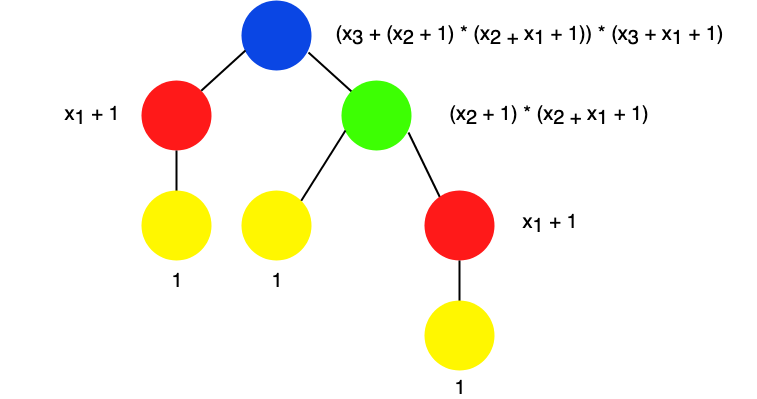
\includegraphics[width=12cm]{figuras/treeIsomorphism.png}
  \caption{Example of a tree with the hash of each node. }
\end{figure}
